\section{Emergent Behaviours}

\subsection{Different Graph Topologies}

The rewiring algorithm \cite{aamas2010} was ran on graphs with a random topology, such as those graphs generated by the Erdos-Renyi generator.
We ran our implementation of this rewiring algorithm on scale-free and small-world graphs.
Scale-free and small-world graphs are a better representation of social networks than random graphs.
In social networks, each user is likely to belong to one or more cliques.
Large numbers of the users in a clique are likely to be connected.
This clique nature creates a number of clusters in the topology, which is different from random topologies where clusters are uncommon.

When we ran these same algorithms on the scale-free and small-world graphs, generated randomly using the JUNG Barab\'{a}si-Albert and Kleinberg Small-world generators, we found that the donation rate remained at a similar level.
Our results show that there is no significant effect on the donation rate with different graph topologies.
Figure \ref{fig:donation-rates-scale-and-small-world} shows as an example, the average donation rates observed on random, scale-free, and small-world graphs against average degree.
The results in this graph used a population size of 200 agents and employed the individual replace worst rewiring strategy, however we found similar behaviour exhibited in all our tests.

\begin{figure}[htbp]
	\centering
	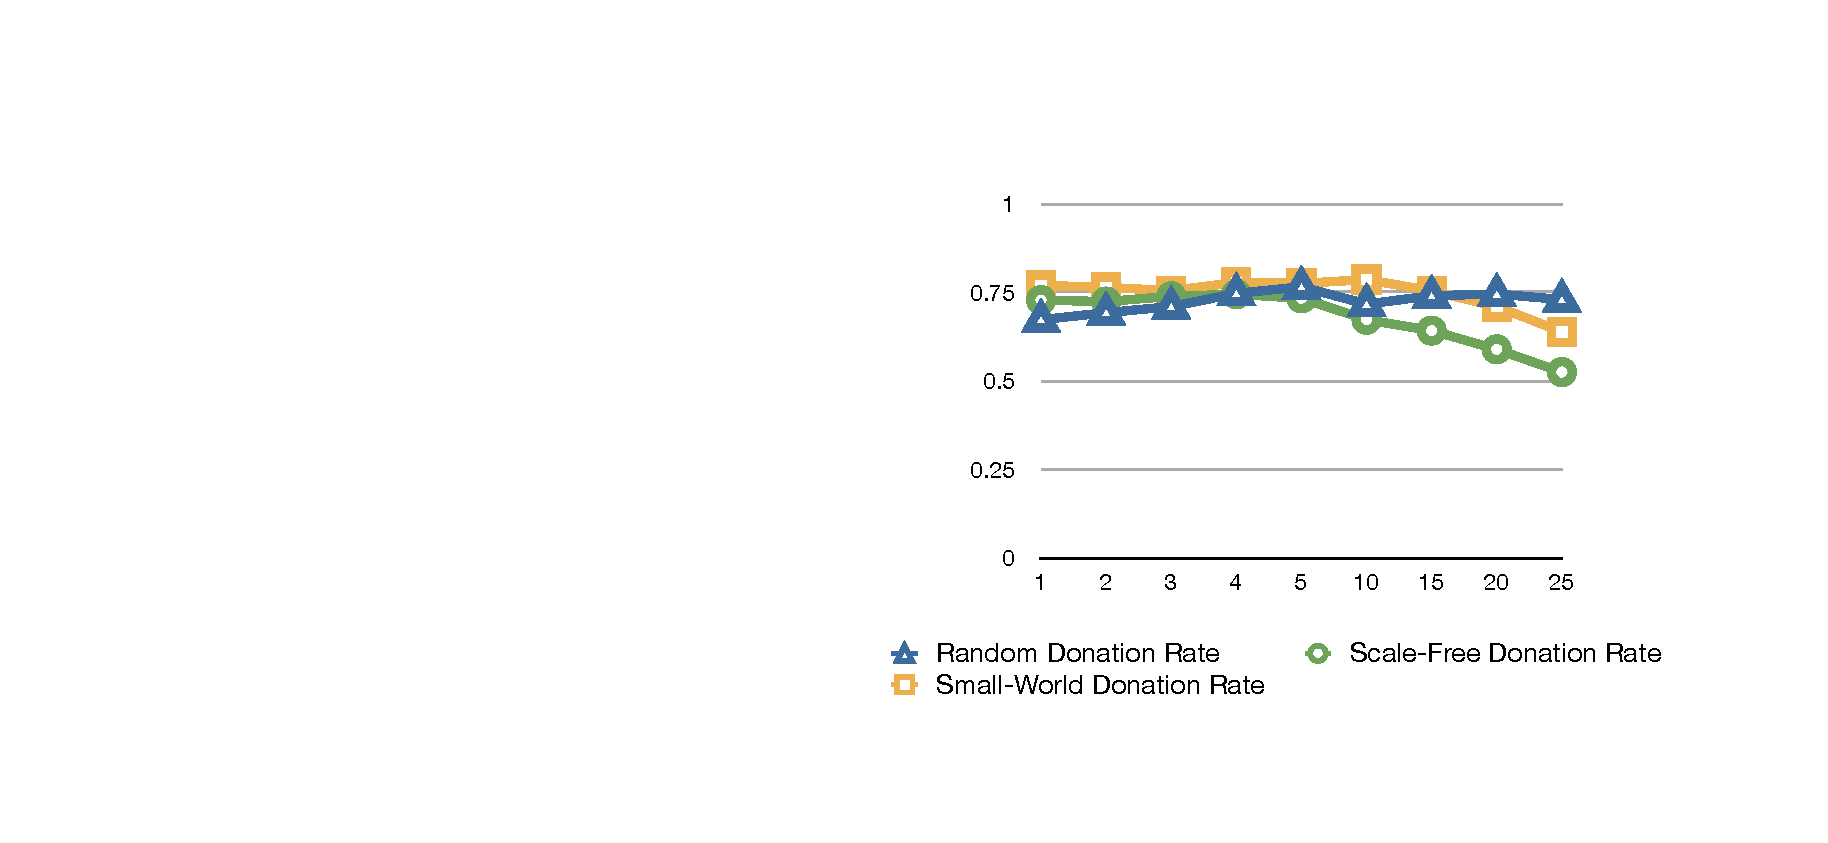
\includegraphics[width=0.7\linewidth]{img/small_world_scale_free_donation_rates.pdf}
	\caption{Donation rates against average degree}
	\label{fig:donation-rates-scale-and-small-world}
\end{figure}

We examined the topological changes caused by the rewiring of the graphs and noticed that although the initial topology was small-world and scale-free, the rewiring caused the topology to morph into a graph with a random topology within just a few generations.

\subsection{Retaining Initial Topological Nature}

We decided that we should look at preserving the initial topological nature of the graphs throughout the simulation, so we decided to look at alternative methods of rewiring that could manage to maintain a similar topology but preserve a donation rate as high as the current rewiring algorithms.

To this end, we decided to create an algorithm that attempts to maintain the same number of small-world connections and long-distance connections during the rewiring. This was achieved by measuring the shortest path length between two neighbours after the neighbour has been removed and then attempting to find a neighbour that has a similar shortest path length to add.

We created two algorithms, the first would be based on the random rewiring strategy and was designed in order to test how the topology changes over time. This differs from the random rewiring strategy in two ways. When a neighbour is about to be removed, the shortest path length between the two agents is measured and stored. Next, when the agent begins to add neighbours to replace those it has removed, it will pick an agent at random and calculate the length of the shortest path between the agent and the random agent, adding a connection only if the length of the shortest path between these two agents is similar to the length of the shortest path between the agent and its neighbour which was removed.

The second algorithm is based on the group replace worst algorithm. Like the algorithm above, when a neighbour is removed, it measures the shortest path between the two agents. Unlike the above algorithm, it then uses an approach based on the group replace worst algorithm to add new nodes. It will query its best neighbours for their best neighbours and will only add a connection to these new agents if the length of the shortest path between them is similar to the length of the shortest path between the agent and its neighbour which was removed.

The results in figure show the impact that these new rewiring algorithms have on the donation rate. It can be seen in these graphs that the new donation rate for the random algorithm performs similarly to that of the existing random rewire algorithms. It can also been seen that the algorithm based on the group replace worst also exhibits similar behaviour to that of the existing group replace worst algorithm.

The results in figure show how the topology changes over time. These results show that the end topology is much closer in nature to the original topology than with the existing rewiring strategies.